\documentclass[13pt,a4paper]{article}
\usepackage[spanish,es-nodecimaldot]{babel}	% Utilizar español
\usepackage[utf8]{inputenc}					% Caracteres UTF-8
\usepackage{graphicx}						% Imagenes
\usepackage[hidelinks]{hyperref}			% Poner enlaces sin marcarlos en rojo
\usepackage{fancyhdr}						% Modificar encabezados y pies de pagina
\usepackage{float}							% Insertar figuras
\usepackage[textwidth=390pt]{geometry}		% Anchura de la pagina
\usepackage[nottoc]{tocbibind}				% Referencias (no incluir num pagina indice en Indice)
\usepackage{enumitem}						% Permitir enumerate con distintos simbolos
\usepackage[T1]{fontenc}					% Usar textsc en sections
\usepackage{amsmath}						% Símbolos matemáticos
\usepackage[ruled,vlined]{algorithm2e}      % Pseudocódigo
\usepackage{xcolor}
\usepackage{listings}
% Para que acepten tíldes los listing
\lstset{     
     literate=%
         {á}{{\'a}}1
         {é}{{\'e}}1
         {í}{{\'i}}1
         {ó}{{\'o}}1
         {ú}{{\'u}}1
         {Á}{{\'A}}1
         {É}{{\'E}}1
         {Í}{{\'I}}1
         {Ó}{{\'O}}1 
         {Ú}{{\'U}}1
         {ñ}{{\~n}}1 
         {Ñ}{{\~N}}1 
         {¿}{{?``}}1 
         {¡}{{!``}}1
}
\usepackage{dsfont}

% ==============================================================================

\usepackage{caption, subcaption}
\usepackage[section]{placeins}
\makeatletter
\def\fps@figure{H}
\makeatother

\usepackage{booktabs}
\usepackage{longtable}
\usepackage{array}
\usepackage{multirow}
\usepackage{wrapfig}
\usepackage{colortbl}
\usepackage{pdflscape}
\usepackage{tabu}
\usepackage{threeparttable}
\usepackage{threeparttablex}
\usepackage[normalem]{ulem}
\usepackage{makecell}
\usepackage{xcolor}
\usepackage[bottom]{footmisc}

\makeatletter
\newcommand*{\centerfloat}{%
  \parindent \z@
  \leftskip \z@ \@plus 1fil \@minus \textwidth
  \rightskip\leftskip
  \parfillskip \z@skip}
\makeatother

% ==============================================================================
% ==============================================================================

% Comando para poner el nombre de la asignatura
\newcommand{\asignatura}{Emprendimiento y transferencia del conocimiento}
\newcommand{\autor}{Ignacio Vellido Expósito}
\newcommand{\email}{ignaciove@correo.ugr.es}
\newcommand{\titulo}{Robot mascota para perros}
\newcommand{\subtitulo}{Trabajos}

% Configuracion de encabezados y pies de pagina
\pagestyle{fancy}
\lhead{\autor{}}
\rhead{\asignatura{}}
\lfoot{Máster Ciencia de Datos e Ingeniería de Computadores}
\cfoot{}
\rfoot{\thepage}
\renewcommand{\headrulewidth}{0.4pt}		% Linea cabeza de pagina
\renewcommand{\footrulewidth}{0.4pt}		% Linea pie de pagina

% ==============================================================================
% ==============================================================================

\usepackage[final]{pdfpages}
\newcommand\invisiblesection[1]{%
  \refstepcounter{section}%
  \addcontentsline{toc}{section}{\protect\numberline{\thesection}#1}%
  \sectionmark{#1}}

\begin{document}
    \pagenumbering{gobble}
    % ==============================================================================
% Pagina de titulo
\begin{titlepage}
    \begin{minipage}{\textwidth}
        \centering

        
\includegraphics[scale=0.5]{img/ugr.png}\\

        \textsc{\Large \asignatura{}\\[0.2cm]}
        \textsc{MÁSTER CIENCIA DE DATOS E INGENIERÍA DE COMPUTADORES}\\[1cm]

        \noindent\rule[-1ex]{\textwidth}{1pt}\\[1.5ex]
        \textsc{{\Huge \titulo\\[0.5ex]}}
        \textsc{{\Large \subtitulo\\}}
        \noindent\rule[-1ex]{\textwidth}{2pt}\\[2.5ex]

        \end{minipage}

        \vspace{0.3cm}

        \begin{minipage}{\textwidth}

        \centering

        \textbf{Autor}\\ {\autor{} \\ ignaciove@correo.ugr.es}\\[1.5ex]
        \vspace{0.4cm}

        
\includegraphics[scale=0.3]{img/etsiit.jpeg}
        
\includegraphics[scale=0.6]{img/master.png}

        \vspace{0.7cm}
        \textsc{Escuela Técnica Superior de Ingenierías Informática y de Telecomunicación}\\
        \vspace{1cm}
        \textsc{Curso 2020-2021}
    \end{minipage}
\end{titlepage}
% ==============================================================================
    
    \pagenumbering{arabic}
    \tableofcontents
    \thispagestyle{empty}				% No usar estilo en la pagina de indice

    \newpage

    % ==============================================================================

    % •    Desarrollo de una propuesta sencilla de plan inicial (modelo de negocio) utilizando el método CANVAS + DAFO.
    % •    Realización de una ficha de búsqueda de financiación empresarial.
    % •    Ejercicio práctico de búsqueda de patentes.
    % •    Realización en casa de un video individual (“Elevator Pitch” de menos de 5 minutos) grabado por cada estudiante, presentando su idea de negocio.
    % •    Realización de una tabla con previsiones financieras
    % •    Ejercicio de desarrollo de creatividad y de liderazgo.

    \section{Modelo CANVAS}

% Aquí una imagen

% 9 campos del canvas y explicarlos

% Canvas (esquema y describirlo, en presentación quizás)

\subsection{Segmento de clientes}

% SC-­‐ Segmento de clientes: grupos de personas o entidades a las que dirigimos las propuestas de valor. ¿Para quien creamos valor? ¿Nos dirigimos a uno o a diferentes segmentos? (Mercado de masas, nicho de mercado, mercado segmentado) . 

La app se puede dirigir a cualquier grupo de personas que posean un móvil, pero debemos tener en cuenta que el problema que pretende resolver puede ser vergonzoso o ridículo para gran parte de la población.

Por tanto, debemos enfocarnos en diferentes tipos de público objetivo que permitan (volver normal) y arrancar el negocio. Estos son:
\begin{itemize}
    \item \textbf{Turistas}: Estando en una ciudad desconocida y sentir la necesidad puede ser un problema grande. Si con el tiempo es posible alcanzar un rango de efectividad semi-global este sector podrá ser muy prometedor.
    \item \textbf{Trabajadores en la calle}: En este sector englobamos personas tales como taxistas, transportistas (camioneros), y cualquier tipo de persona que se desplace constantemente en sus horarios de trabajo. La probabilidad de uso de la aplicación por parte de este grupo de usuarios es menor pues gran parte de ellos ya conocerán lugares donde ir al servicio. Aunque nuestra app probablemente tengo un uso más esporádico, la inclusión de estimación de ocupación e higiene puede ser útil para este grupo de personas.
    \item \textbf{Usuarios con problemas intestinales}: Principal público objetivo. Al ser conscientes de su enfermedad tendrán hábitos y preocupaciones que los inciten a usar la aplicación, con la idea de tener el máximo de información es sus decisiones (por ej: un usuario puede usar la información para decidir dónde comer si cree que va a tener una urgencia tras la comida).
\end{itemize}

\subsection{Propuesta de valor}

% PV-­‐ Propuestas de valor: productos y servicios que crean valor para un segmento de mercado específico. El obje8vo es solucionar los problemas de los clientes: “Qué quiere comprar nuestro cliente" versus "qué vendemos". 

Proponemos información detallada y a tiempo real de los mejores lugares en los que ir al baño para nuestros usuarios. Para tenemos en cuenta no solo las preferencias del cliente (nivel de urgencia, localización) sino también la calidad de los posibles lugares (higiene, ocupación).

Todo esto además se ofrece de manera gratuita para el usuario.

\subsection{Canales de comunicación, distribución y venta}

% C-­‐ Canales de comunicación, distribución y venta: la forma en que la empresa establece contacto con los diferentes clientes y cómo les proporciona la propuesta de valor. 

% Anuncios en redes sociales, Youtube. Se espera que a la larga la manera que resulte más eficiente sea el boca-a-boca.

% Soporte mediante una página web ?

\subsection{Relación con los clientes}

% RC-­‐ Relación con los clientes: relaciones de la empresa con cada segmento de clientes. En función de cada cliente, adaptaremos el discurso.

\subsection{Ingresos}

% I-­‐Ingresos: se generan cuando los clientes compran las propuestas de valor que ofrece la empresa. ¿Por qué valor pagarían nuestros clientes? ¿Cómo pagan ahora? ¿Cómo les gustaría pagar? 

Se podría considerar añadir información extra tras algunos modelos de pago, pero es esencial que la funcionalidad principal se ofrezca gratuítamente al usuario si queremos alcanzar fidelidad con ellos. Esto nos deja con dos posibles formas de ganar ingresos:

\begin{itemize}
    \item Anuncios de manera no intrusiva, de forma que no empeoremos la opinión de los usuarios.
    \item Venta de datos.
\end{itemize}

\subsection{Recursos y capacidades}

% RC-­‐Recursos y capacidades clave: acFvos necesarios para el modelo de negocio, incluidas las personas de la empresa y sus capacidades (Recursos esicos, intelectuales, humanos, y económicos). 

\begin{itemize}
    \item Servidores y bases de datos que soporten el sistema. Preferiblemente contratado mediante un modelo SaaS.
    \item Personal de desarrollo, soporte, y reparación de la aplicación ante posibles caídas.
    \item Personal legal y de recursos humanos ?
\end{itemize}

\subsection{Actividades clave}

% AC-­‐Ac8vidades clave: acciones necesarias que deben llevarse a cabo si contamos con las capacidades y recursos necesarios (Producción, I+D, Resolución de problemas, Plataforma..) 

\subsection{Partners clave}
% Google y Apple ?

% PC -­‐ Partners (Alianzas) clave: las alianzas, los socios, incluso los proveedores que necesitamos para el éxito del modelo de negocio. Algunas acFvidades se pueden externalizar. 

Se podrían usar mapas de software libre.
En otro caso, si quisiéramos usar las APIs de Google y Apple, deberíamos tener una buena relación con ellos.

\subsection{Estructura de costes}

% EC-­‐ Estructura de costes: gastos asociados a la puesta en marcha de un negocio para poder elaborar y hacer llegar la propuesta de valor a los clientes (Costes fijos, variables, low-­‐cost, según valor, economias de escala,..)

El coste de los recursos tecnológicos tendrá una base fija y una variable en función de la demanda de usuarios y el rango de soporte (países) de la aplicación.
Existe también un coste de distribución en las tiendas de software móvil (App Store y Play Store)

Coste fijo del personal técnico y (legal?) \newpage
    \section{Análisis DAFO}  

\begin{figure}[H]
    \centering
    \makebox[\textwidth][c]{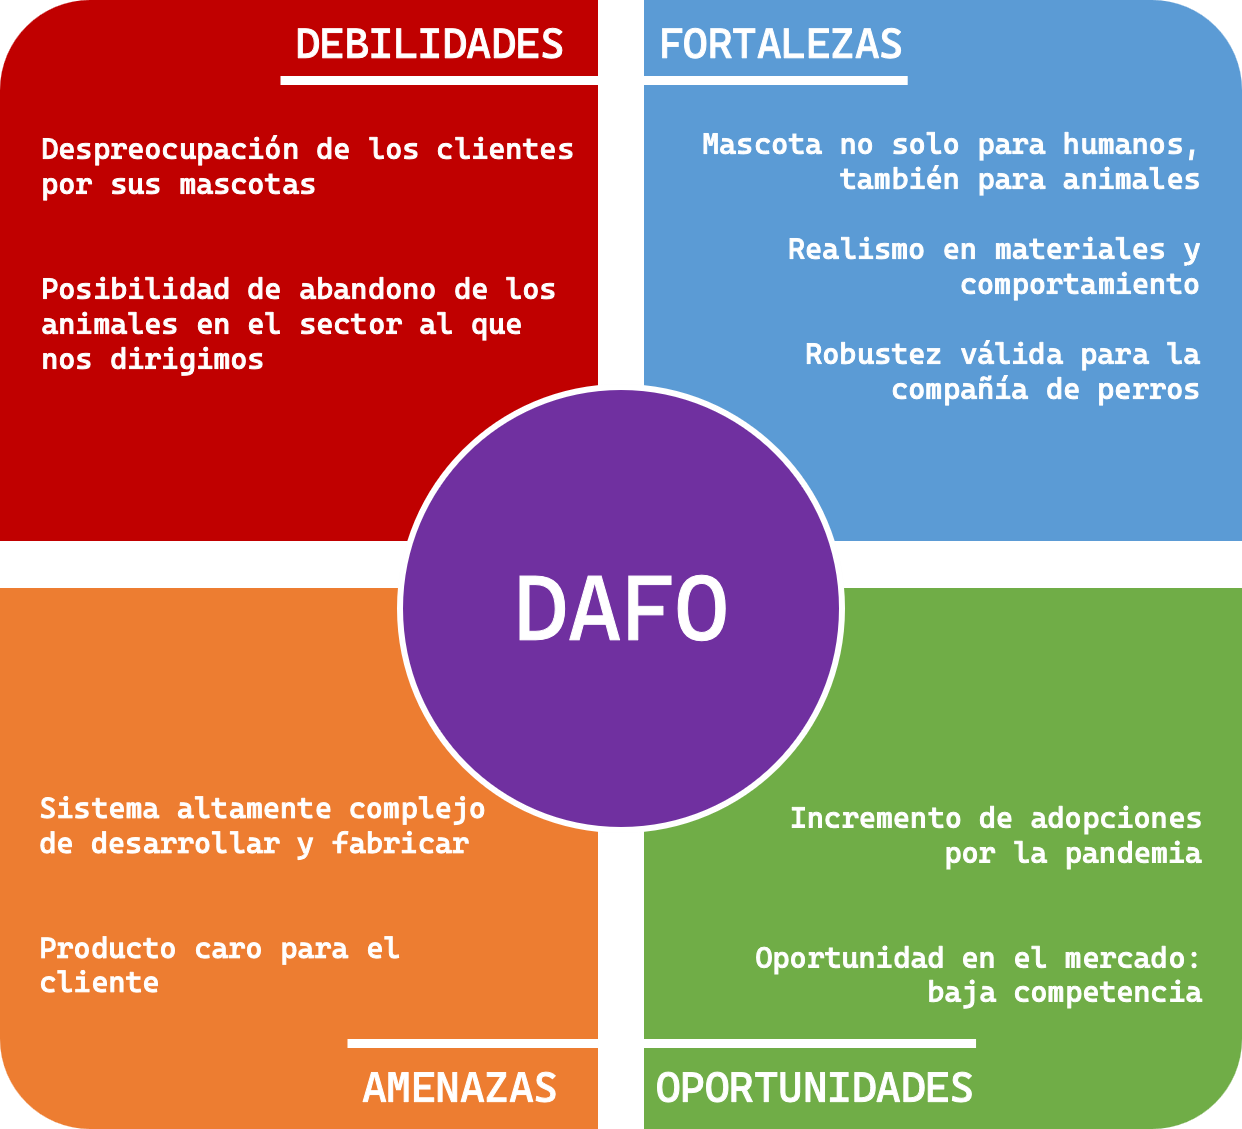
\includegraphics[width=.8\textwidth]{img/dafo.png}}%
\end{figure}

\subsection{Fortalezas}
% • Qué ventajas tiene nuestra empresa (o idea inicial) sobre la competencia (técnicas, de costes, de experiencia, de recursos humanos, .. 
% • Qué elementos perciben nuestros clientes como una fortaleza de empresa 
% • Cual es el know-­‐how de nuestros recursos humanos 
% • Donde está nuestra innovación 

Nosotros proponemos un robot cuadrúpedo que haga que la mascota se encuentra frente ``a un igual'', de forma que juegue y se comunique con él al igual que lo haría con otro perro. De esta forma nos diferenciamos de la mayoría del mercado, centrado en robots de compañía para humanos y no para mascotas. 

Investigando la competencia solo hemos encontrado un principal competidor en este segmento. Frente a ellos, su falta de proporciones similares a un perro (el suyo es un robot clásico estilo roomba) y nuestro realismo en olor y textura hará que nuestro modelo alcance más fácilmente el cariño tanto de la mascota como del dueño.

\subsection{Debilidades}
% • Qué hace peor nuestra empresa que la competencia 
% • En qué procesos somos más lentos o ineficientes 
% • Qué perciben nuestros clientes como debilidades 
% • Qué aspectos tecnológicos del sector aún no hemos incorporado 
% • Qué nos dificulta adaptarnos a las peFciones de nuestros clientes 

El producto a desarrollar es extremadamente complejo y costoso. Necesitamos proveer de sistemas sensoriales, motores e intelectuales que ``confundan'' a una máquina por un animal (en principio, desde la perspectiva de la mascota). El sistema debe ser robusto y seguro, lo que conlleva mucho tiempo de investigación y testeo.
Todo esto se resume en que contaríamos con un proceso pre-producción largo y caro.

\vspace{\baselineskip}

Esto nos obligará a demostrar con mayor énfasis nuestra propuesta de valor frente a la competencia y las ventajas de la inversión.

\subsection{Oportunidades}
% • Qué tendencias favorables presenta el mercado 
% • Qué necesidades de los clientes no están cubiertas por la competencia 
% • Qué cambios legislaFvos posiFvos se han producido o se prevén 
% • Qué hábitos de vida o de infraestructuras han cambiado y pueden favorecer al sector 

Los robots enfocados a perros en la actualidad carecen de facultades realistas que permitan que el animal empatice de forma más profunda. La mayoría vagamente pasan del umbral de ``juguetes con ruedas'' y buscan más paliar el servicio de proporcionar comida que de acompañar. Además sabemos que una gran parte de los dueños de mascotas están dispuestos a gastar grandes cantidades de dinero por el bienestar tanto físico como emocional del animal.

\vspace{\baselineskip}

Por otro lado, la masiva adopción de perros por la pandemia en hogares/familias que no estaban preparados para ello acaba con los animales gran parte del día solos en casa o incluso abandonados, ya que tras el levantamiento de los confinamientos los dueños vuelven a la rutina y están poco tiempo presentes en la casa. Nuestro robot mascota aporta entretenimiento y compañía para los animales durante estas horas de ausencia.

% https://www.kickstarter.com/projects/51244428/mia-a-friendly-robot-for-cats-and-dogs-by-kolony-r

\subsection{Amenazas}
% • Qué cambios tecnológicos que yo no dispongo están sucediendo en el mercado 
% • Qué hábitos de consumo se prevén que puedan reducir el mercado 
% • Qué tendencias demográficas pueden perjudicar al sector 
% • Cual es la situación del sector financiero 
% • Qué acuerdos internacionales pueden perjudicarnos 

La posibilidad de abandono de las mascotas en los hogares de estos posibles clientes puede reducir significativamente el mercado. Adicionalmente, la gran cantidad de financiación necesaria y lo complejo del desarrollo puede dejarnos sin recursos económicos antes de lanzar el robot en producción. \newpage
    \invisiblesection{Financiación}
    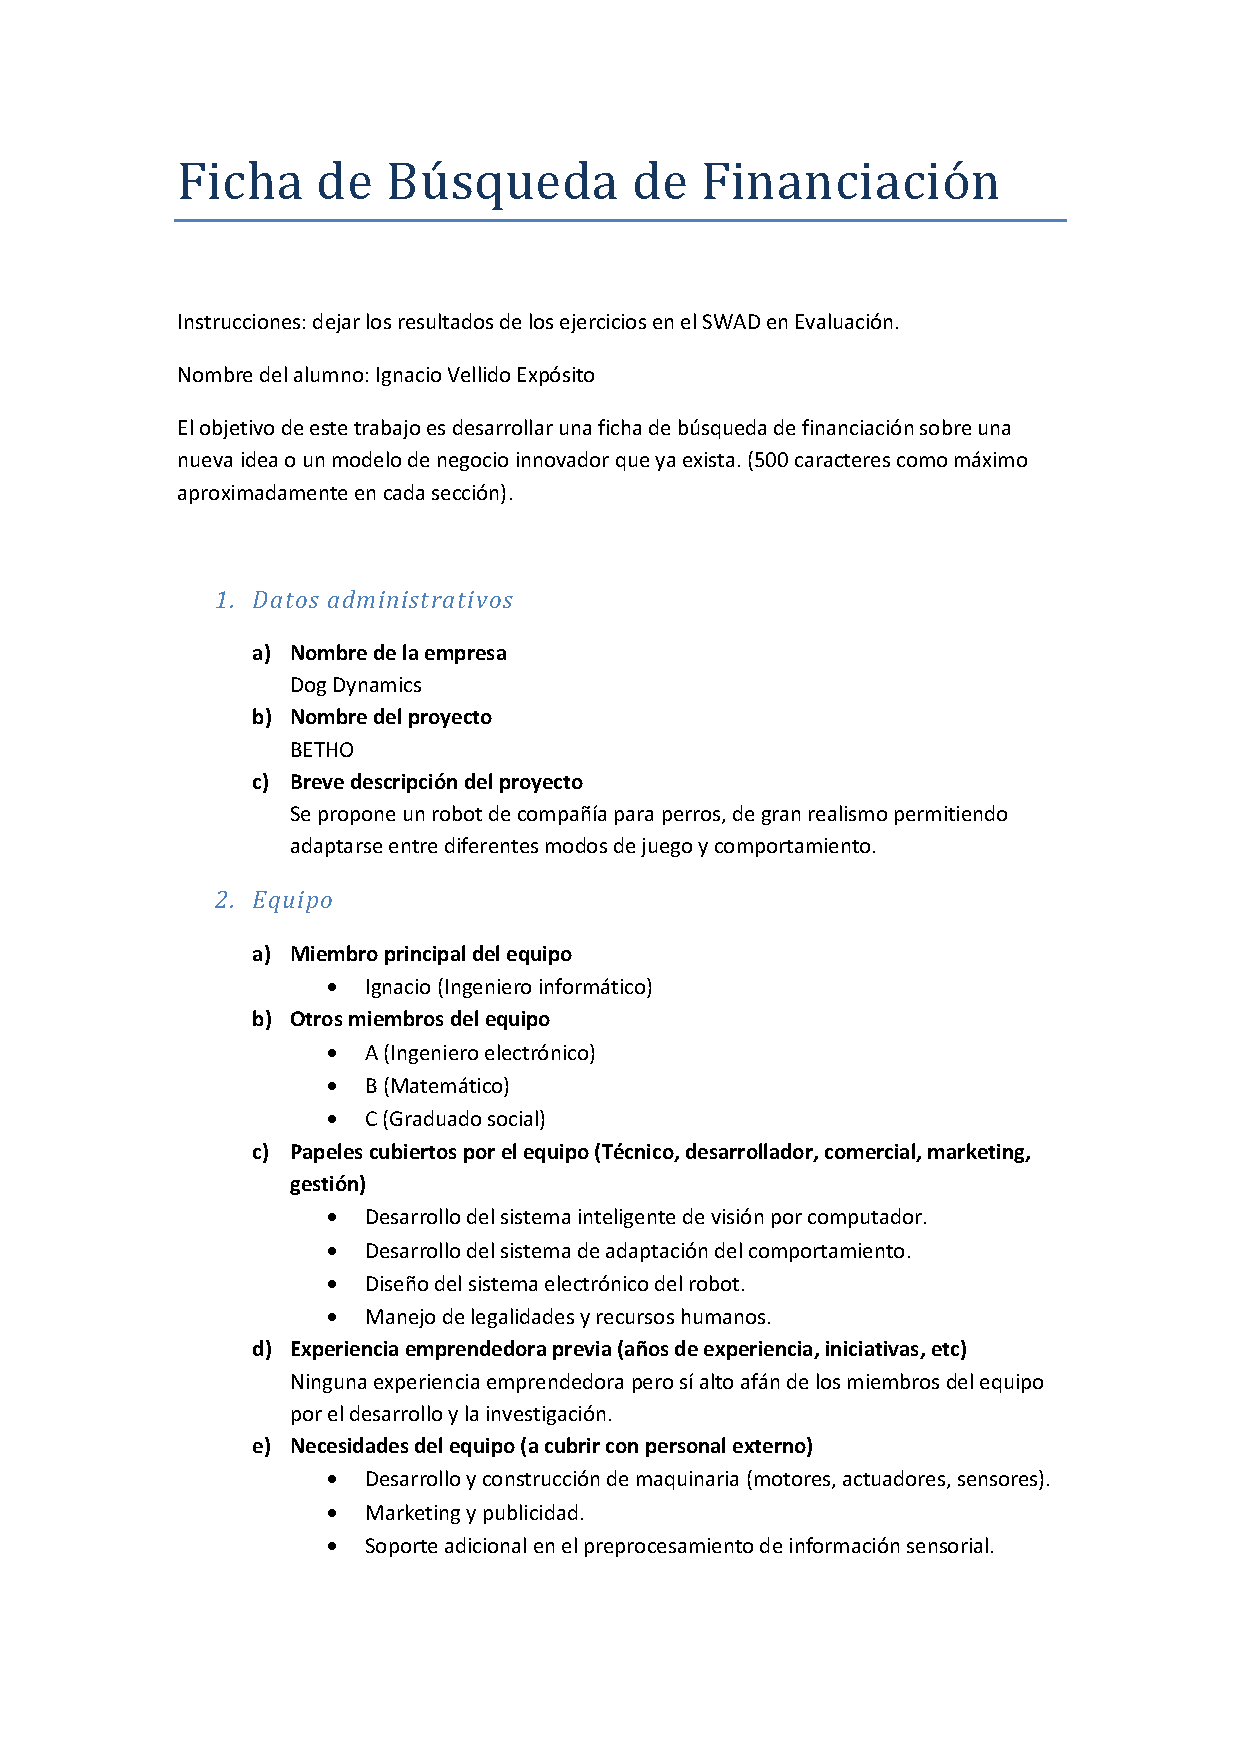
\includepdf[pages=-]{Ficha_Busqueda_Financiacion.pdf}
    \section{Patentes}

\subsection{}

Buscar patentes de relacionadas con el campo de vuestra idea de negocio (por ejemplo patentes relacionadas con redes neuronales, patentes relacionadas con lógica difusa, etc. Si vuestra idea de negocio o tecnología se relaciona con “soft-computing”). Buscar con palabras clave (key words).

\par\noindent\rule{\textwidth}{0.4pt}

He buscado patentes a partir de las keywords ``robot dog''.

\begin{itemize}
    \item ¿Cuántas son?. Utilizando LENS indicar con un gráfico cómo es la evolución de patentes en este campo.
    
    \begin{itemize}
        \item LENS: 20.846 patentes.
        \item Google patents: 75.624 patentes.
        \item Espacenet: 13.335 patentes.
    \end{itemize}
    
    \begin{figure}[H]
        \centering
        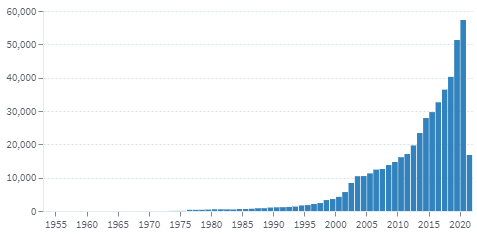
\includegraphics[width=.8\textwidth]{img/patentes/2a.png}
    \end{figure}

    Mirando por encima no todas patentan un robot al completo. Muchas de ellas describen sistemas de visión, sistemas de control, circuitos\dots.

    \item Identificar algún código de clasificación de patentes (CPC o CIP) relacionado.
    
    He visto 2 códigos CPC frecuentemente:
    \begin{itemize}
        \item A63H11/00: Derivado de salud y juguetes.
        \item B25J19/00: Para sistema de control de manipuladores.
    \end{itemize}

    \item Indicar número de patentes de ese código (CPC o CIP).
    \begin{itemize}
        \item A63H11/00: 5.396 patentes.
        \item B25J19/00: 48.745 patentes.
    \end{itemize}

    \item Indicar las tres principales empresas que tienen patentes relacionadas con ese código (CPC o CIP).
    \begin{itemize}
        \item A63H11/00: Sony Corp (636), Mattel INC (172), Groove X INC (95).
        \item B25J19/00: Fanuc LTD (1.164), Seiko Epson Corp (590), Kawasaki Heavy Industries (461).
    \end{itemize}

    \item Buscar una patente en concreto e indicar el link donde aparezcan los “claims” (o reivindicaciones) de una patente en este campo.
    
    Patente CN205273661U:

    \url{https://worldwide.espacenet.com/patent/search/family/056058262/publication/CN205273661U?q=pn%3DCN205273661U}
\end{itemize}


\subsection{}

A la hora de valorar patentes se puede tener en cuenta el crecimiento del área tecnológica, que a su vez se puede medir de forma indirecta analizando el crecimiento registrado en el número de solicitudes de patente en un área específica de la tecnología, valorando positivamente aquellas tecnologías cuyas patentes hayan registrado un crecimiento continuado en el pasado reciente (20 años) frente a las que hayan registrado un crecimiento negativo, discontinuo o alejado en el tiempo.

Buscar tendencias de patentes en las siguientes temáticas (utilizar el buscador “LENS”).

Para cada caso añadir el gráfico de tendencia anual de patentes sobre esta temática (gráfico de número de patentes por año relacionadas con ese campo):

\par\noindent\rule{\textwidth}{0.4pt}

\begin{itemize}
    \item Buscar patentes sobre “Face recognition”. Indicar cuántas tiene “Samsung” sobre esta temática

    498.029 patentes. 10.504 de Samsung.

    \begin{figure}[H]
        \centering
        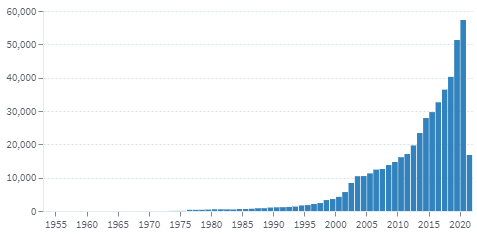
\includegraphics[width=.8\textwidth]{img/patentes/2a.png}
    \end{figure}

    \item Buscar patentes sobre “Fuzzy logic”. Indicar cuántas tiene “Microsoft” sobre esta temática.

    96.435 patentes. 4.696 + 2.141 del conglomerado de empresas de Microsoft.

    \begin{figure}[H]
        \centering
        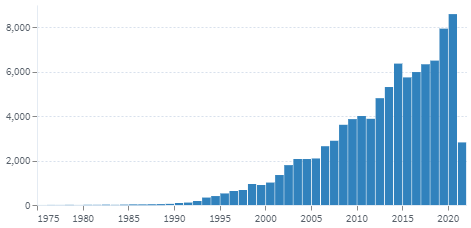
\includegraphics[width=.8\textwidth]{img/patentes/2b.png}
    \end{figure}

    \item Buscar patentes sobre “SVM” (Support Vector Machine). Indicar cuántas tiene “Microsoft” sobre esta temática.
    
    504.121 patentes. 6.829 + 5.415 del conglomerado de empresas de Microsoft.

    \begin{figure}[H]
        \centering
        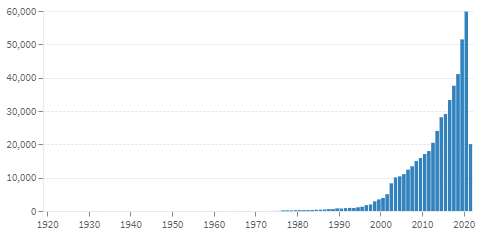
\includegraphics[width=.8\textwidth]{img/patentes/2c.png}
    \end{figure}
\end{itemize}

\subsection{}

Búsqueda de una patente y relación con patentes similares. Por ejemplo con Google Patents o Espacenet.

Buscar la patente WO2020033205A1. Indicar: 
\begin{itemize}
    \item \textbf{Los Inventores}: Stephen Alan Mckinley, David Gealy y Pieter Abbeel.
    \item \textbf{Institución o persona que realiza la solicitud}: Universidad de California.
    \item \textbf{Fecha de la solicitud}: 2019-07-31.
    \item \textbf{Fecha de la publicación}: 2020-02-13.
    \item \textbf{Códigos de Clasificación (CPC)}:
    \begin{itemize}
        \item B25J18/00 (US) 
        \item B25J9/0087 (EP)
        \item B25J9/102 (EP)
        \item B25J9/126 (EP,US)
        \item F16H48/38 (US) 
        \item B25J19/06 (US)
        \item F16H2048/387 (US)
    \end{itemize}
\end{itemize}


% Patentes
% 1) Quizás desarrollar un poco
% 2) Solo el número y (opcional) una gráfica
% 3) Solo las preguntas

% https://worldwide.espacenet.com/patent/search/family/069228268/publication/WO2020033205A1?q=WO2020033205A1 \newpage
    \section{Creatividad y liderazgo}

% En estas sesiones se proponen ejercicios (denominados entregables) que deben realizarse y ser entregados en un documento pdf.
% Para la entrega en SWAD (zona mis trabajos), se requiere
% – Extensión mínima: 1 página + portada
% – Extensión máxima: 3 páginas + portada
% – La portada debe indicar el nombre del (los) alumno(s) así como su titulación.
% – Letra del texto: Arial 11, interlineado simple
% – Letra de los títulos: Arial 13 (negrita)

\subsection{Entregable 1}
% De la lista de empresas fracasadas disponible en https://www.cbinsights.com/blog/startup-failure-post-mortem/ seleccionen como mínimo una empresa (puede elegir más) y comente el porqué de su fracaso. Discusión: ¿hay solapamientos o paralelismos?

Se elige la empresa \textit{Starsky Robotics}, centrada en el ámbito de conducción autónoma y, más concretamente, la de camiones de transporte. Entre los principales motivos del fracaso, se indica la pérdida de financiación una vez que los problemas a la hora de cumplimentar el objetivo de la empresa se volvieron aparentes. A pesar de pequeños éxitos, la lentitud del despliegue operativo de camiones autónomos en empresas con poca base tecnológica supuso un impedimento enorme para la startup.

\vspace{\baselineskip}

Adicionalmente, el proceso repetitivo (pero necesario) de validación del sistema para mantener la seguridad en carretera tiene poco gancho para los inversores, pues retrasa la promesa de beneficios. Por otro lado, la competencia atraía la atención pública (en contraposición a ellos) creando funcionalidades extremadamente modernas, pero con mucho camino para un uso fiable.

\vspace{\baselineskip}

También se achaca el problema a que la empresa surgió demasiado pronto y no alcanzó el momentum necesario para mantenerse en el largo camino que queda para conseguir una conducción 100\% autónoma.

% https://medium.com/starsky-robotics-blog/the-end-of-starsky-robotics-acb8a6a8a5f5

% Title: The End of Starsky Robotics

% Product: Starsky Robotics

% Starsky Robotics, an autonomous trucking tech startup, folded in March 2020. In a blog post, CEO Stefan Seltz-Axmacher outlined the reasons the company had failed, stating:

% Timing, more than anything else, is what I think is to blame for our unfortunate fate. Our approach, I still believe, was the right one but the space was too overwhelmed with the unmet promise of AI to focus on a practical solution. As those breakthroughs failed to appear, the downpour of investor interest became a drizzle.


\subsection{Entregable 2}
% – Listar varias “tecnologías”, escoger al azar una. Escoger al azar sustantivo y un adjetivo (sencillos)
% – Proponer un producto o servicio basándonos en la tupla generada aleatoriamente. Tupla de ejemplo (Drones, brazo, amarillo)

% \begin{itemize}
%     \item Aerogel
%     \item Grafeno
%     \item Laser
%     \item Textiles electrónicos
%     \item Turbina
%     \item Batería
%     \item Televisión
%     \item Escáner
%     \item Radio
%     \item Radar
%     \item Armas
%     \item Satélite
%     \item Vehículo % Transporte
% \end{itemize}

\textbf{Nota}: Me gustó la idea que salió y la he querido desarrollar con el resto de ejercicios de la asignatura.

\vspace{\baselineskip}

Usando la página \url{https://www.palabrasaleatorias.com/} se generan las siguientes tuplas:
\begin{itemize}
    \item (cachorro, Holanda)
    \item (anécdota, bingo)
    \item (vivir, reja)
\end{itemize}

\vspace{\baselineskip}

Propongo el siguiente producto a partir de la primera tupla:

\vspace{\baselineskip}

Las cuarentenas impuestas en los países del norte de Europa (como Holanda, Dinamarca, Suecia\dots) debido a la pandemia actual han generado un aumento repentino en el número de adopciones de perros. 
Una vez pasados los confinamientos y la vuelta al trabajo estos animales se encuentran (en el mejor de los casos) separados de sus dueños durante la mayor parte del día, afectándo negativamente su salud mental por la falta de interacción social, sobre todo en los cachorros de baja edad.

\vspace{\baselineskip}

Para solucionar este problema proponemos un nuevo tipo de robot cuadrúpedo que se ``comunica'' y juega con perros. Gracias a un buen sistema de computación visual, el robot es capaz de reconocer el estado de ánimo del cachorro y adaptar su comportamiento, cambiando entre diferentes modos de juego y compañía. Adicionalmente, el robot es programable y en base a la edad del cachorro asimila un comportamiento más materno. También es capaz de almacenar un mapa virtual de la casa y mantener al animal en las habitaciones que desee el dueño.


\subsection{Entregable 3}
% – Haga la prueba de Hersey-Blanchard y comente su resultado.

\subsubsection{Herser-Blanchard test}

Mis respuestas han sido: 1.A 2.A 3.A 4.D 5.C 6.D 7.B 8.A 9.C 10.D 11.B 12.D

Dándome como resultado en amplitud de estilos:
\begin{itemize}
    \item Directivo: 3
    \item Persuasivo: 5
    \item Participativo: 3
    \item Delegativo: 1
\end{itemize}

Y en adaptabilidad de estilos:
\begin{itemize}
    \item Directivo: 0
    \item Persuasivo: -1
    \item Participativo: 2
    \item Delegativo: 18
    \item \textbf{Suma}: 19
\end{itemize}

Siendo más altos de lo que me esperaba en persuasivo, pero me cuadra en participativo. Siento que mi perspectiva es ``si algo funciona bien, mejor dejarlo'' e intentar involucrar a todos y que se sientan contentos (pero sin dejar de aportar al equipo). El alto valor en directivo lo achaco a que aunque intentaría ser flexible y amigable, siendo líder soy responsable de mis subordinados, y por ello dependo de sus buenos resultados.

Sobre la adaptabilidad, los resultados me concuerdan ya que considero que cada uno es ``experto'' en lo suyo y por tanto su opinión es tan válida como la del líder. Es este último el que debe escuchar, pero en última instancia valorar y decidir.

\subsubsection{Liderazgo situacional}

% – Escriba una reflexión sobre cómo ha aplicado o echado en falta la aplicación de un liderazgo situacional en su vida profesional (académica en su defecto). Nota: si usted no ha sido jefe/líder, escriba sobre su experiencia como subordinado.

Aunque no está dentro del ámbito profesional me gustaría hablar de mi experiencia personal como líder situacional en mi vida social. 
Para poner en situación, pertenezco a un grupo de 4 amigos con una buena costumbre de elegir cuidadosamente los regalos de cumpleaños. La cosa está en que soy el único del grupo preocupado por prever los regalos con antelación y no acabar entregándolos después de tiempo, por lo que suelo asumir el puesto de organizador todos los años.

\vspace{\baselineskip}

Uno de ellos es menos afán de regalos materiales, y siento un rol más participativo cuando propongo y coordino la realización de regalos hechos por nosotros, intentando que se note el cariño de cada uno.

El rol delegativo se ve con el segundo de ellos, puesto que al tener una amistad más afín con un amigo y menos con el resto del grupo suelo indicarle que investigue sobre posibles ideas.

El liderazgo directivo no lo veo en este contexto, pero por el test de Herser-Blanchard tampoco parece que sea muy frecuente en mi persona.

\vspace{\baselineskip}

Luego, desde mi punto de vista como subordinado (como jugador en un equipo de voleibol), he sentido que los entrenadores suelen carecer de liderazgo situacional, comportándose únicamente como delegativo cuando las rachas eran buenas y directivos en las malas. La inclusión de liderazgo persuasivo creo que habría ayudado a subir la moral en aquellas épocas de torneos, y el participativo para considerar la opinión de todo el equipo, muchas veces ignorada, aunque desde el punto de vista de un jugador en ocasiones vemos las cosas con más facilidad.

% Mencionar los cuatro tipos de liderazgo

% Entrega 3, cuestionario en SWAD (hacerlo es opcional)
% La reflexión solo vale. Líder en lo que sea propia (amigos ? trabajos de universidad?)
% Sino subordinado identificando los 4 estilos de liderazgo (Identificarlo siempre)



% • Distribución
% • Servicio
% • Compra
% • Transporte
% • Formación
% • Garantías

% ¿Por qué mi producto o servicio es mejor?
% • ¿Cómo conseguir que me compren a mí?
% • ¿Cómo puedo sobrevivir a la competencia futura?

    % ==============================================================================

    \setlength{\parskip}{1em}
    \newpage
    % \nocite{*}
    % \bibliography{bibliografia}
  	% \bibliographystyle{plain}
\end{document}